% Image -> latent grid -> index grid -> sequence — TikZ source. Compiles to a
% tight standalone PDF (pdflatex figures/grid-sequence.tex), which
% `book-scaffold build-figures` converts to public/figures/grid-sequence.svg.
%
% An image is encoded to an L-cell latent grid; each cell is quantized to a
% codebook index; reading the index grid in raster order gives a length-L
% sequence over {1,...,K} — a sentence in the visual vocabulary.
\documentclass[tikz,border=3pt]{standalone}
\usepackage{amsmath}
\usepackage{amssymb}
\usepackage{tikz}
\usetikzlibrary{positioning,arrows.meta,calc}
\begin{document}
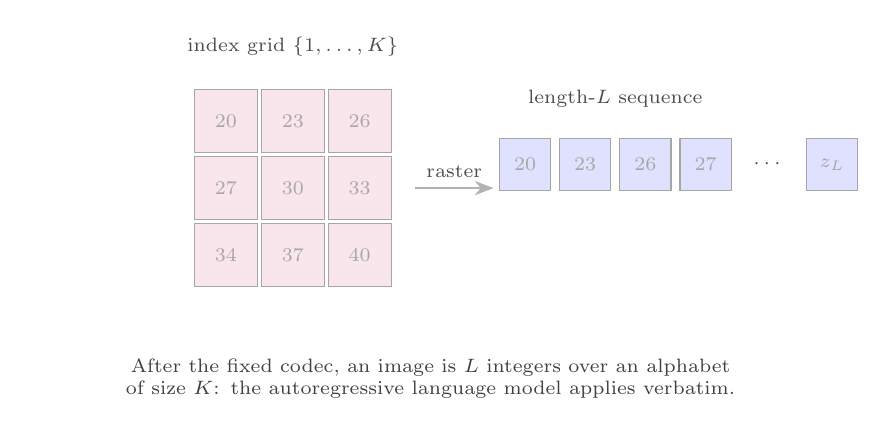
\begin{tikzpicture}[
    font=\small,
    op/.style={->, >={Stealth[length=2.4mm]}, gray!60, thick},
    tok/.style={draw, gray!70, fill=blue!12, minimum size=6.5mm, inner sep=1pt,
                font=\scriptsize},
  ]
  % latent grid (3x3) of indices
  \begin{scope}
    \foreach \r in {0,1,2}
      \foreach \c in {0,1,2} {
        \pgfmathtruncatemacro{\idx}{int(20+\r*7+\c*3)}
        \node[draw, gray!70, fill=purple!10, minimum size=8mm, inner sep=1pt,
              font=\scriptsize] at (\c*0.85, -\r*0.85) {\idx};
      }
    \node[above, font=\scriptsize, text=black!70] at (0.85,0.7)
      {index grid $\{1,\dots,K\}$};
  \end{scope}

  % arrow to sequence
  \draw[op] (2.4,-0.85) -- (3.4,-0.85)
    node[midway, above, font=\scriptsize, text=black!70] {raster};

  % flattened sequence (first few tokens)
  \begin{scope}[shift={(3.8,-0.55)}]
    \node[tok] (s0) {20};
    \node[tok, right=1mm of s0] (s1) {23};
    \node[tok, right=1mm of s1] (s2) {26};
    \node[tok, right=1mm of s2] (s3) {27};
    \node[right=1.5mm of s3, font=\scriptsize, text=black!70] (dots) {$\cdots$};
    \node[tok, right=1.5mm of dots] (sl) {$z_L$};
    \node[above, font=\scriptsize, text=black!70] at ($(s1)!0.5!(s2)+(0,0.6)$)
      {length-$L$ sequence};
  \end{scope}

  \node[below, align=center, text width=10cm, font=\scriptsize, text=black!75]
    at (2.6,-2.9)
    {After the fixed codec, an image is $L$ integers over an alphabet of size $K$:
     the autoregressive language model applies verbatim.};
\end{tikzpicture}
\end{document}
